\documentclass[spanish,letterpaper,oneside]{article}

\def\documenttitle {Construyendo aprendizaje a través de habilidades}
\def\documentsubtitle {Temas selectos de matemáticas I · Cohorte SD26}
\def\documentsubject {Actividad 4 (Sesión 11) · Reporte de Lectura: SEP (1994) y Alsina (2023)}
\def\documentauthor {Mtro. Martín Jonathan de la Cruz Muñoz}
\def\coursename {Temas selectos de matemáticas I}
\def\coursecode {PFM02}

\def\universityname {Instituto de Investigación, Innovación y Estudios de Posgrado para la Educación del Estado de Nuevo León}
\def\universityfaculty {Maestría en Aprendizaje y Enseñanza de las Matemáticas}
\def\universitydepartment {Temas selectos de matemáticas I}
\def\universitydepartmentimage {img/iiiepe/marca-iiiepe.png}
\def\universitydepartmentimagecfg {height=1.75cm}
\def\universitylocation {Monterrey, Nuevo León}
\def\studentfullname {Mtro. Martín Jonathan de la Cruz Muñoz}
\def\studentid {00874}
\def\studentemail {martin.delacruz@campus.iiiepe.edu.mx}
\def\programperiod {2do periodo, agosto--noviembre de 2026 (SD26)}
\def\programmodality {Modalidad presencial y en línea}
\def\programshort {MAEM}

\def\authortable {
  \begin{tabular}{ll}
    \textbf{Alumno:} & \studentfullname \\
    Matrícula: & \studentid \\
    Correo institucional: & \studentemail \\
    Unidad: & \coursename \\
    Programa: & \programshort \\
    Periodo: & \programperiod \\
    & \\
    \multicolumn{2}{l}{Fecha de realización: 31 de octubre de 2026} \\
    \multicolumn{2}{l}{\universitylocation}
  \end{tabular}
}

\input{template}

\usepackage{helvet}
\renewcommand{\familydefault}{\sfdefault}
\usepackage{amsmath,amssymb,booktabs,array,longtable,pdflscape,tikz,tabularx,colortbl,pgfplots,enumitem,needspace}
\usepackage[most]{tcolorbox}
\usetikzlibrary{arrows.meta,positioning,calc,fit,backgrounds,babel}
\pgfplotsset{compat=1.18}

\definecolor{iiiepeNavy}{HTML}{163B5C}
\definecolor{iiiepeBlue}{HTML}{1F6F9F}
\definecolor{iiiepeAqua}{HTML}{20B7A8}
\definecolor{iiiepeOrange}{HTML}{F28C28}
\definecolor{iiiepePaper}{HTML}{F6F8F7}
\definecolor{iiiepeInk}{HTML}{1E2A32}
\definecolor{iiiepePale}{HTML}{EEF5F8}
\def\portraittitlecolor {iiiepeNavy}
\setcitestyle{authoryear,open={(},close={)}}

\newcommand{\insertcoverwatermark}{%
  \AddToShipoutPictureBG*{%
    \begin{tikzpicture}[remember picture,overlay]
      \node[opacity=.06,inner sep=0pt] at (current page.center)
      {
\includegraphics[width=.58\paperwidth]{img/iiiepe/logo-puntos.png}};
    \end{tikzpicture}%
  }%
}

\newtcolorbox{propuestabox}[1][]{%
  enhanced,breakable,
  colback=iiiepePaper,colframe=iiiepeAqua!80!iiiepeNavy,
  boxrule=1pt,leftrule=4pt,arc=2pt,
  left=8pt,right=8pt,top=6pt,bottom=6pt,
  before skip=6pt,after skip=10pt,
  fonttitle=\bfseries\color{white},coltitle=white,
  colbacktitle=iiiepeNavy,
  attach boxed title to top left={xshift=8pt,yshift=-2pt},
  boxed title style={colback=iiiepeNavy,colframe=iiiepeNavy,arc=1pt},
  title={Propuesta didáctica},#1}

\setlength{\parskip}{5pt}\setlength{\parindent}{0pt}
\begin{document}\insertcoverwatermark\templatePortrait\templatePagecfg\templateFinalcfg\fancyfoot{}\fancyfoot[L]{\scriptsize IIIEPE · MAEM · SD26}\fancyfoot[C]{\scriptsize\thepage}\fancyfoot[R]{\scriptsize Actividad 4}\setstretch{1.25}\raggedbottom

\section{Introducción}
El desarrollo del pensamiento matemático en la escuela secundaria y media superior exige articular las ocho habilidades operatorias, comunicativas y heurísticas descritas en el enfoque didáctico de la \citet{sep1994} con la resolución de problemas genuinos como eje articulador planteado por \citet{alsina2023}. A continuación se expone el análisis comparado de ambos marcos, la fundamentación de cinco habilidades prioritarias y su aplicación en un Proceso de Desarrollo de Aprendizaje (PDA) situado.

\section{Apartado A: Análisis articulado de SEP (1994) y Alsina (2023)}

\subsection{Las ocho habilidades matemáticas en SEP (1994, pp. 12--13)}
El \textit{Libro para el maestro. Matemáticas. Educación secundaria} \citep{sep1994} plantea como propósito formativo cardinal desarrollar habilidades operatorias, de comunicación y de descubrimiento en relación dialéctica con actitudes positivas y conocimientos matemáticos. Apoyado en \citet{monereo1998}, dicho enfoque distingue entre \textbf{capacidad} (disposición genética inicial), \textbf{habilidad} (variación individual desarrollada por el uso en un entorno culturalmente organizado) y \textbf{destreza} (agilidad en técnicas manuales); además, sistematiza ocho habilidades matemáticas fundamentales integrando los procesos descritos por \citet{alsina2023}.

\needspace{15\baselineskip}
{\small\setstretch{1.08}\renewcommand{\arraystretch}{1.18}
\noindent\begin{tabularx}{\textwidth}{|>{\raggedright\arraybackslash}p{0.18\textwidth}|>{\raggedright\arraybackslash}X|>{\raggedright\arraybackslash}p{0.31\textwidth}|}\hline
\rowcolor{iiiepePale} \textbf{Habilidad (SEP, 1994)} & \textbf{Definición en el enfoque oficial (pp. 12--13)} & \textbf{Proceso afín en Alsina (2023)} \\\hline
\textbf{1. Calcular} & Establecer relaciones entre cifras o términos de una operación o ecuación para producir o verificar resultados. & Resolución de problemas y pensamiento computacional (algoritmos). \\\hline
\textbf{2. Inferir} & Establecer relaciones entre datos explícitos e implícitos en textos, figuras, tablas, gráficas o diagramas. & Conexiones y razonamiento inductivo. \\\hline
\textbf{3. Comunicar} & Utilizar simbología y conceptos matemáticos para interpretar y transmitir información cualitativa y cuantitativa. & Comunicación y representación matemática. \\\hline
\textbf{4. Medir} & Establecer relaciones entre magnitudes para calcular longitudes, superficies, volúmenes o masas. & Modelización y representación de magnitudes. \\\hline
\textbf{5. Imaginar} & Trabajo mental de idear trazos, formas y transformaciones geométricas planas y espaciales. & Representación y visualización espacial. \\\hline
\textbf{6. Estimar} & Encontrar resultados aproximados de medidas, operaciones, ecuaciones y problemas. & Razonamiento heurístico y supervisión (Pólya). \\\hline
\textbf{7. Generalizar} & Descubrir regularidades, reconocer patrones y formular procedimientos y resultados generales. & Pensamiento computacional (patrones/abstracción) y modelización. \\\hline
\textbf{8. Deducir} & Establecer hipótesis y encadenar razonamientos para demostrar teoremas sencillos. & Razonamiento y prueba matemática. \\\hline
\end{tabularx}}
\vspace{4pt}

\subsection{La resolución de problemas según Alsina (2023, pp. 71--75)}
\citet{alsina2023} plantea que las prácticas matemáticas competenciales deben abandonar la memorización mecánica de algoritmos para centrarse en la interpretación matemática del entorno. En sus tres conocimientos esenciales sobre la resolución de problemas destaca: (1) distinguir entre \textit{ejercicio} (aplicar una técnica conocida) y \textit{problema} (situación genuina sin camino expedito, abierta al ensayo y análisis); (2) diversificar las tipologías de problemas; y (3) acompañar pedagógicamente las \textbf{cuatro fases heurísticas de \citet{polya1945}}: comprensión del problema, planificación de estrategias, ejecución y supervisión, evitando la ayuda directiva que anula la autonomía del estudiante \citep{alsina_planas2008}.

\subsection{Relación dialéctica entre ambos textos}
Ambos documentos convergen en una tesis medular \citep{sep1994,alsina2023}: los problemas no constituyen un apéndice final para ejercitar procedimientos previos, sino el \textbf{motor epistémico} que detona las habilidades matemáticas. Mientras el enfoque oficial operacionaliza ocho habilidades acompañadas de actitudes de indagación y perseverancia, la propuesta contemporánea incorpora procesos transversales y preguntas guía de mediación docente. Además, dado que una habilidad solo se consolida frente a retos con incertidumbre, es decir, cuando el estudiante coordina representaciones múltiples y argumenta sus conclusiones, ambos marcos se complementan recíprocamente; sin embargo, su implementación exige transformar la gestión del aula y, por tanto, superar la enseñanza meramente expositiva.

\begin{center}
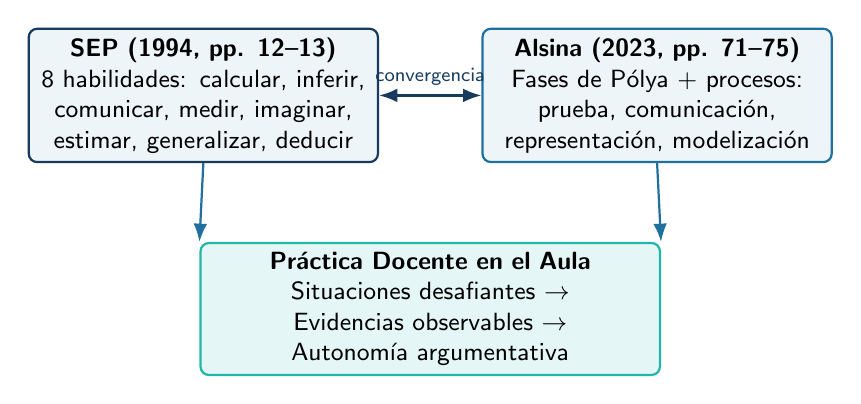
\begin{tikzpicture}[font=\small,node distance=1.3cm,>=Latex]
  \node[draw=iiiepeNavy,fill=iiiepePale,thick,rounded corners=3pt,text width=4.2cm,align=center] (sep) {\textbf{SEP (1994, pp. 12--13)}\\8 habilidades: calcular, inferir, comunicar, medir, imaginar, estimar, generalizar, deducir};
  \node[draw=iiiepeBlue,fill=iiiepePale,thick,rounded corners=3pt,text width=4.2cm,align=center,right=of sep] (als) {\textbf{Alsina (2023, pp. 71--75)}\\Fases de Pólya + procesos: prueba, comunicación, representación, modelización};
  \node[draw=iiiepeAqua,fill=iiiepeAqua!12,thick,rounded corners=3pt,text width=5.6cm,align=center,below=1.0cm of $(sep.south)!0.5!(als.south)$] (aula) {\textbf{Práctica Docente en el Aula}\\Situaciones desafiantes $\rightarrow$ Evidencias observables $\rightarrow$ Autonomía argumentativa};
  \draw[<->,thick,iiiepeNavy] (sep) -- node[above,font=\scriptsize] {convergencia} (als);
  \draw[->,thick,iiiepeBlue] (sep.south) -- (aula.north west);
  \draw[->,thick,iiiepeBlue] (als.south) -- (aula.north east);
\end{tikzpicture}
\end{center}

\section{Apartado B: Selección y justificación de cinco habilidades prioritarias}
Desde mi experiencia docente en bachillerato tecnológico (CONALEP) y educación superior en ingeniería, selecciono las cinco habilidades prioritarias siguientes:
\begin{enumerate}
  \item \textbf{Inferir:} \textit{Importancia:} Los problemas técnicos y cotidianos rara vez entregan todos los datos ordenados en una ecuación; el estudiante debe leer planos, tablas o gráficas e identificar restricciones implícitas. \textit{En resolución de problemas:} Al interpretar una gráfica de fuerzas o consumo, el alumno extrae relaciones no declaradas literalmente antes de operar.
  \item \textbf{Comunicar:} \textit{Importancia:} Expresar procedimientos con lenguaje simbólico y argumentación verbal consolida la comprensión profunda y expone errores conceptuales que el resultado numérico oculta. \textit{En resolución de problemas:} Se activa al redactar la justificación de un diseño en equipos y defender por qué un procedimiento es válido frente a soluciones alternativas.
  \item \textbf{Estimar:} \textit{Importancia:} Previene la aceptación ciega de resultados absurdos arrojados por la calculadora y desarrolla sentido numérico y de magnitud. \textit{En resolución de problemas:} En la fase de comprensión y supervisión (Pólya), el alumno acota órdenes de magnitud antes de calcular y valida si su respuesta final es físicamente razonable.
  \item \textbf{Generalizar:} \textit{Importancia:} Permite transitar de casos particulares numéricos al pensamiento algebraico y la modelización funcional, evitando que cada problema nuevo parezca aislado. \textit{En resolución de problemas:} Tras ensayar 3 o 4 casos en una tabla, el estudiante formula una regla explícita aplicable a cualquier valor futuro.
  \item \textbf{Deducir:} \textit{Importancia:} Forma el pensamiento matemático crítico descrito por Alsina y Planas (2008): cuestionar afirmaciones, encadenar propiedades conocidas y probar por qué algo se cumple siempre. \textit{En resolución de problemas:} Permite demostrar una fórmula o descartar una conjetura falsa sin depender de la validación del profesor.
\end{enumerate}

\section{Apartado C: Vinculación con la práctica docente (PDA situado)}
\textbf{PDA seleccionado (MCCEMS · Pensamiento Matemático / CONALEP):} \textit{``Resuelve problemas de variación proporcional directa en sistemas físicos y tecnológicos, modelando algebraicamente la relación fuerza--área, interpretando la constante de proporcionalidad y validando con tabla y gráfica''.}

\textbf{Situación trabajada:} Análisis de una prensa o excavadora hidráulica donde un émbolo menor de diámetro $d_1$ recibe una fuerza $F_1$ y se busca la fuerza resultante $F_2$ en un émbolo mayor de diámetro $d_2 = 2 d_1$.
\begin{itemize}
  \item \textbf{Habilidades matemáticas desarrolladas:} \textit{Inferir} (deducir que la presión se transmite íntegra por el Principio de Pascal), \textit{Calcular y Medir} (evaluar áreas circulares $A = \pi r^2$), \textit{Estimar} (anticipar si $F_2$ será mayor al doble de $F_1$), \textit{Generalizar} (obtener $F_2 = k\cdot F_1$ con $k = (d_2/d_1)^2$) y \textit{Comunicar/Deducir} (justificar por qué duplicar el diámetro cuadruplica la fuerza).
  \item \textbf{Acciones de los estudiantes e intervención docente:} El alumnado construye tablas para distintas relaciones de diámetro, grafica en GeoGebra y contrasta la predicción lineal errónea ($2\times$) contra el modelo cuadrático real ($4\times$). El docente orienta mediante preguntas sin entregar la fórmula de golpe, acompañando las fases de Pólya.
\end{itemize}

\clearpage
\section{Conclusiones y transferencia profesional}
El análisis comparado entre el marco de habilidades matemáticas \citep{sep1994} y la perspectiva competencial contemporánea de resolución de problemas \citep{alsina2023} confirma nuestra tesis central: los desafíos matemáticos no constituyen un apéndice mecánico, sino el entorno epistémico donde las ocho habilidades adquieren sentido verificable. En términos de análisis propio, se advierte que priorizar \textit{Inferir}, \textit{Comunicar}, \textit{Estimar}, \textit{Generalizar} y \textit{Deducir} corrige la tendencia escolar de reducir la matemática a cálculo rutinario, dado que exige justificar cada etapa heurística de \citet{polya1945}.

En consecuencia, el hallazgo más relevante de la vinculación con el sistema hidráulico radica en que el estudiante confronta sus conjeturas intuitivas mediante variación proporcional cuadrática y validación gráfica \citep{alsina_planas2008}. No obstante, para asegurar una aplicación efectiva en el ejercicio profesional del nivel medio superior y superior, resulta indispensable articular evidencias observables con preguntas orientadoras que sostengan la autonomía argumentativa; por ello, el impacto didáctico se potencia al exigir tablas, expresiones simbólicas y verificaciones en aula. Desde una perspectiva analítica propia, considero que articular estas cinco habilidades prioritarias transforma la evaluación en un proceso formativo riguroso, lo cual me lleva a sostener que enseñar desde el desafío mejora sustancialmente la comprensión matemática en el ejercicio profesional docente.

\newsavebox{\hiddenbibbox}
\begin{lrbox}{\hiddenbibbox}\begin{minipage}{\textwidth}\bibliography{referencias}\end{minipage}\end{lrbox}

\end{document}
